\section{Diseño}
A continuación se presentan y explican algunas de las desiciones de diseño elegidas durante el desarrollo del trabajo practico.
Se decidió dividir la presentación en subsecciones para facilitar la comprensión de la misma, haciendo especial énfasis en aquéllas que consideramos son de mayor importancia para la comprensión del mismo.

%Vale mencionar que si bien es cierto que se genero una idea general en el grupo antes de comenzar a reflejar las decisiones tomadas en codigo, el diseño en profundidad se termino de desarrollar y afinar en paralelo, mientras surgian cuestiones mismas relacionadas al propio desarrollo que no habian sido tenidas en cuenta en papel. 


\subsection{Participantes, cap y fichas}
Decidimos que un en un modelado correcto del participante no tenía sentido desde el punto de vista de responsabilidades del objeto que lo represente que conozca su cap (presupuesto para armar equipos) ni su cantidad de fichas disponibles, puesto que no son esenciales. Por lo tanto, diseñamos dos clases, el GestorDeCap y el GestorDeFichas, cuyas instancias son objetos que conocen para un participante dado el cap y la cantidad de fichas disponibles respectivamente, además de proveer un protocolo para la actualización de esos valores, que nos permiten desligar a las instancias de la clase Participante de dichas responsabilidades.\\
El nombre Gestor para ambas clases proviene del hecho de que sus instancias gestionan las fichas/caps de los participantes, no són solo objetos que proveen información, sino que la mantienen también.\\
Instancias de ambas clases se utilizan también en la gestión de desafíos, dado que las apuestas afectan la cantidad de fichas disponibles de un participantes y el resultado de un desafíos afecta no sólo a las fichas disponibles de un participante, sino también a su cap.\\
El GestorDeCap entonces utiliza también la clase Presupuesto, que representa en el contextor del Gestor al presupuesto que un participante tiene como límite a la hora de conformar equipos.\\
Análogamente, el GestorDeFichas utiliza la clase Fichas, que representa una cantidad de fichas dada.\\
Si bien ambas clases parecen representar conceptos parecidos, preferimos organizar el conocimiento en dos clases distintas, para dejar en claro la diferencia existente entre ambas entidades en el dominio del problema.\\

\begin{center}
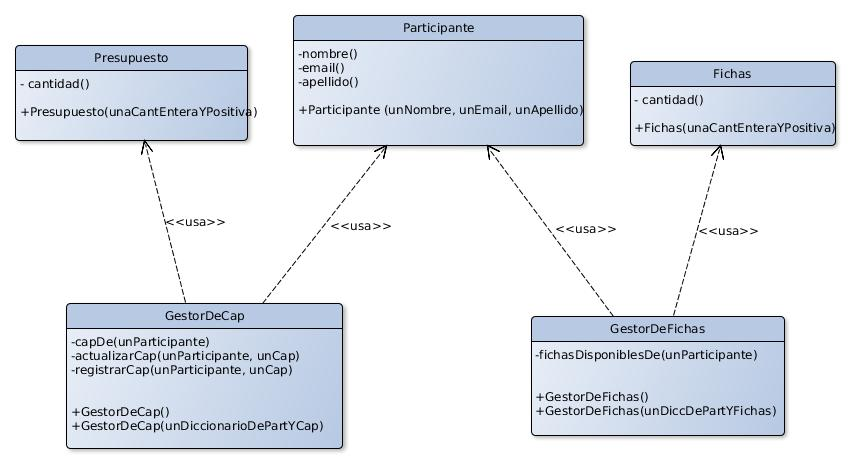
\includegraphics[scale=0.4]{diseno/gestorDeCapYFichas.jpg} 
\end{center}

Finalmente, con el mismo argumento esgrimado en párrafos anteriores, no es esencial al participante conocer directamente sus equipos. Resolvimos esto de una manera similar, como explicaremos en la siguiente subsección.\\


\subsection{Acciones}
Todas las jugadas que pueden desarrollarse durante la simulacion de un partido, se divide claramente en dos grupos. Aquellas que realiza el equipo que esta atacando, y aquellas que realiza aquel que esta defendiendo. En base a esta idea, planteamos nuestro diseño clasificando a todas las acciones que pueden realizarse dentro de una jugada, en alguno de estos dos grupos (Ofensivas y Defensivas) y sub clasificando luego, de acuerdo al tipo de accion.
Este diseño, ademas de presentar de forma simple la realidad, nos permite extender el modelo con nuevas acciones tanto ofensivas como defensivas, de manera relativamente sencilla. Bastaria simplemente con declarar una nueva clase de herede de el tipo de clasificacion correspondiente de la accion. Por supuesto, la accion conoce al jugador que la esta ejecutando para poder mantener la informacion de la simulación de forma consistente.
\begin{center}
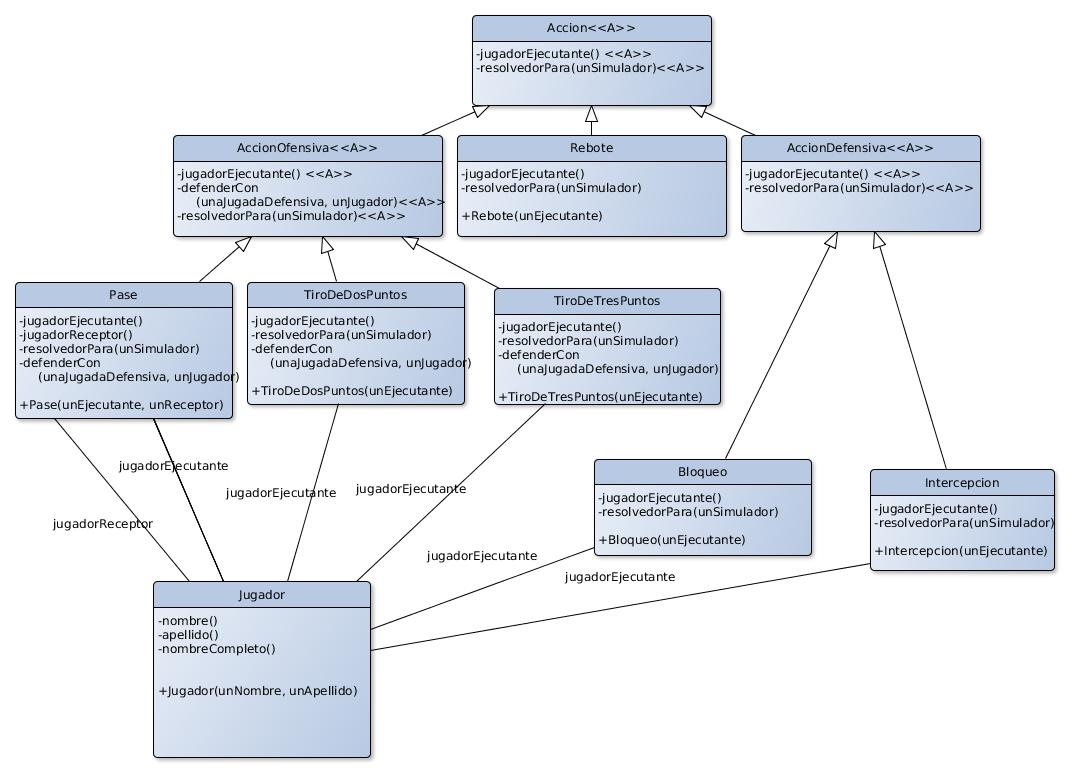
\includegraphics[scale=0.35]{diseno/acciones.jpg}
\end{center}

Veamos entonces como es que estas acciones se elijen y se ejecutan:
\begin{center}
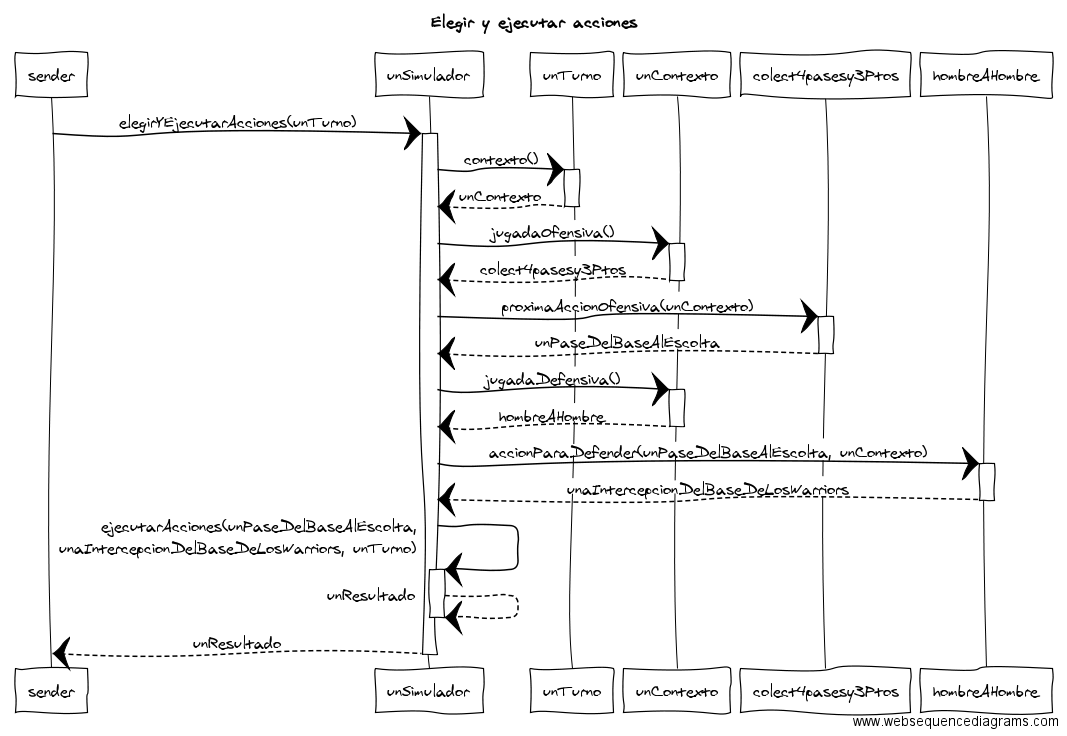
\includegraphics[scale=0.35]{diseno/Elegir_y_ejecutar_acciones.png}
\end{center}
Queda entonces claro como es que el simulador se encarga de tomar la jugada que se esta realizando del contexto y solicitarle las acciones correspondientes a cada una de estas para, luego de recibidas, proceder a ejecutarlas.

\subsection{Jugadas y acciones}
A continuación, presentamos entonces, como es que cada una de las acciones mencionadas en el apartado anterior, se integra con las jugadas defensivas/ofensivas, que componen los libros de los tecnicos.
\begin{center}
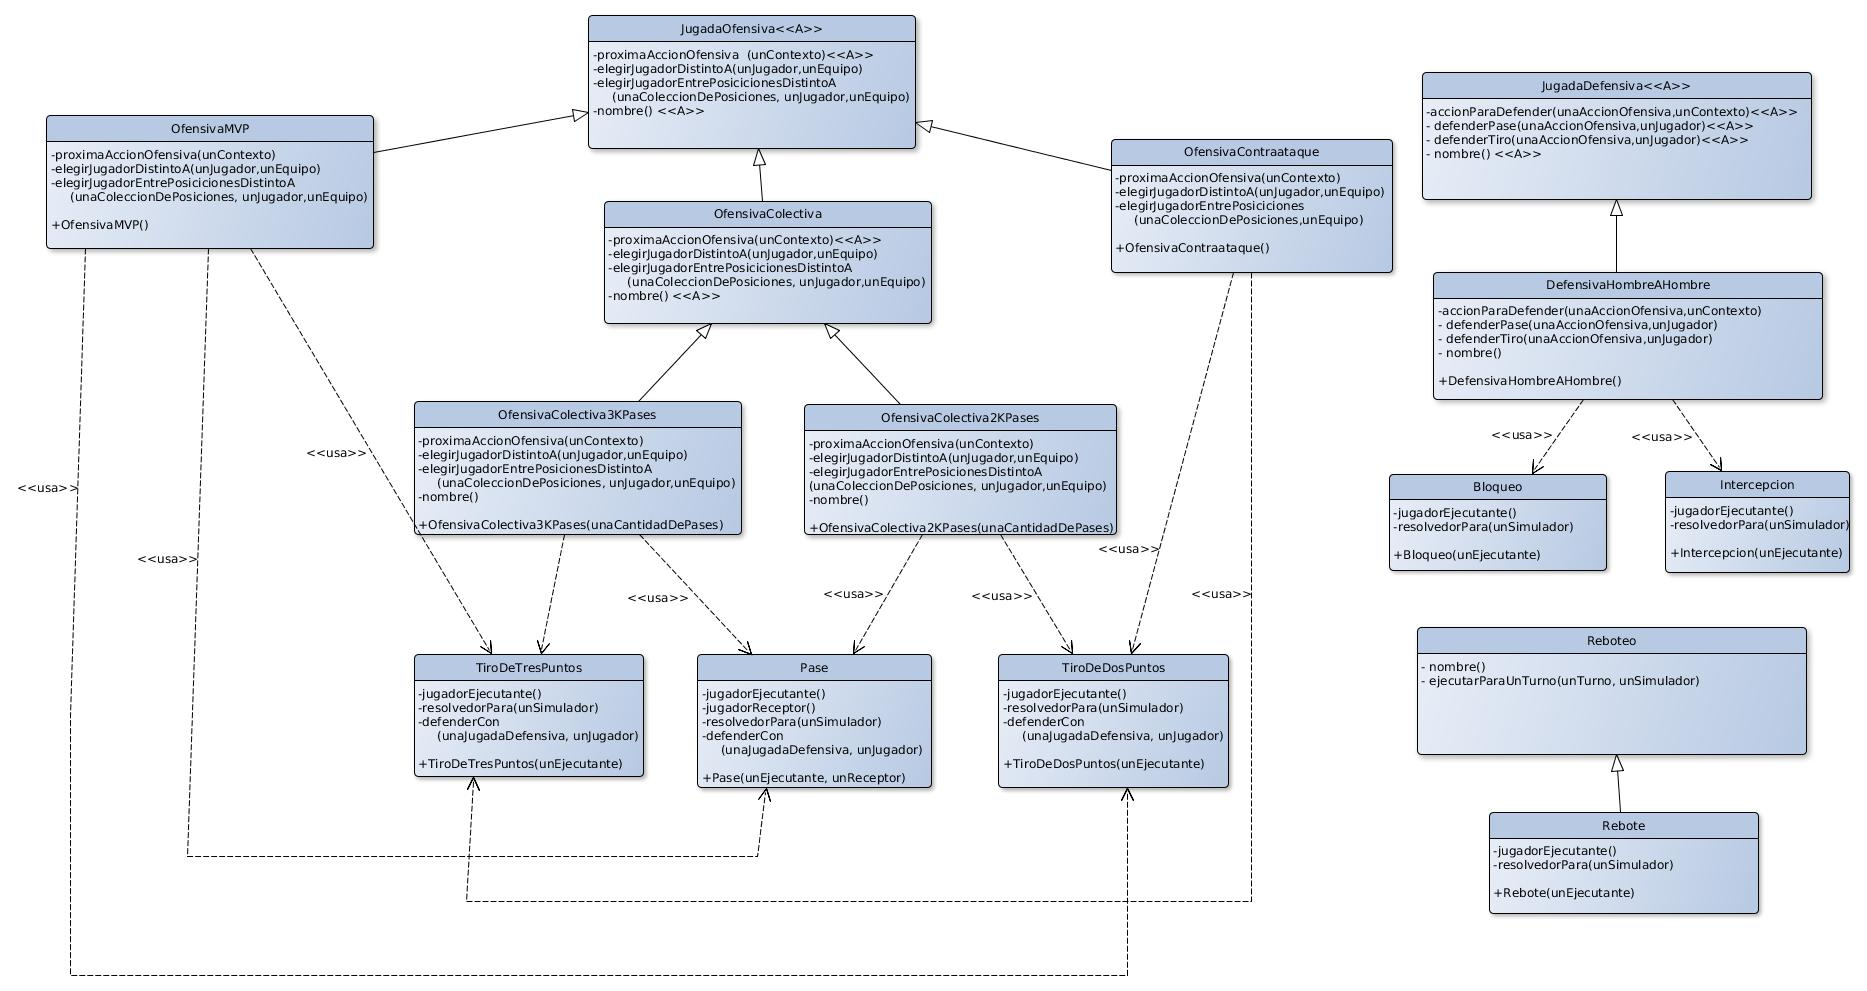
\includegraphics[scale=0.4, angle=90]{diseno/jugadasYAcciones.jpg}
\end{center}

En el siguiente diagrama de secuencia, podremos ver ademas, como estas distintas entidades encargadas de modelar las acciones de una jugada se relacionan con sus propios resolvedores. Estas ultimas son las entidades donde se calculan las distintas posibilidades de exito y fracaso para todas las interacciones entre dos jugadores. El hecho de que estos calculos no sean parte de las acciones en si, nos permite modificar los valores de las ecuaciones encargadas de calcular los resultados de cada accion de forma aislada y sin afectar al resto del modelo.

\begin{center}
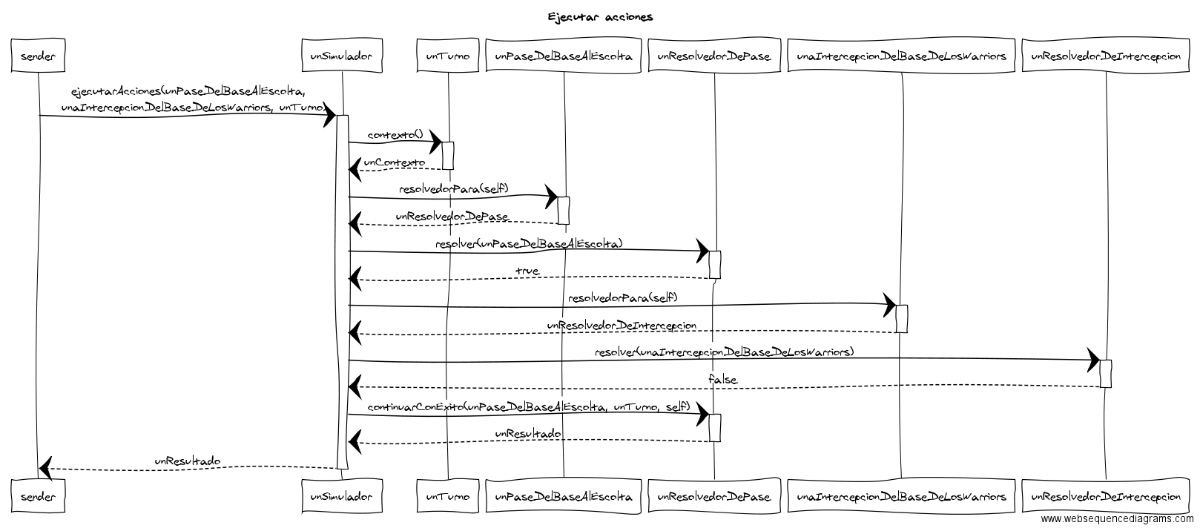
\includegraphics[scale=0.4, angle=90]{diseno/Ejecutar_acciones.png}
\end{center}


\subsection{Apuestas}
Decidimos que la mejor forma de clasificar las apuestas era mediante una jerarquizacion, para poder representar de forma clara que existen aquellas en las que se pone en juego un numero X de fichas, pero tambien aquellas nulas en las que no hay cap apostado. Esta clasificación, si bien es posible que agregue mas complejidad al diseño que suponiendo que las apuestas nulas son aquellas con cantidad de fichas igual a cero, nos ahorra de tener que manejar un unico tipo de apuesta y preguntar por la cantidad de fichas apostados todo el tiempo, permitiendo alijerar el manejo de las apuestas.
\begin{center}
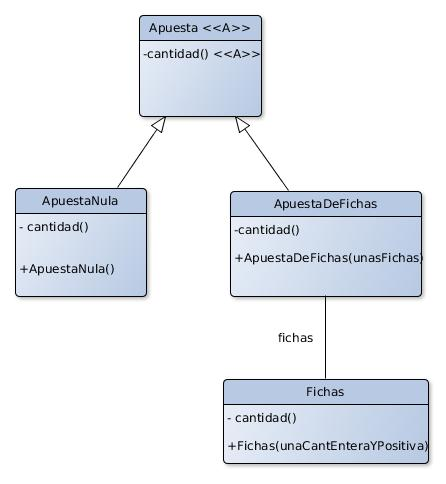
\includegraphics[scale=0.4]{diseno/apuestas.jpg}
\end{center}

\subsection{Equipo, jugadores y tecnico}
Para modelar al equipo, decidimos que exista una clase abstracta posición donde se hereden cada una de las posibles posiciones que puede adoptar un jugador. Nos parecio que es la forma mas correcta de representar la realidad, y si bien es cierto que en el tiempo las posibles posiciones no vayan a variar, nos permite diferenciar a cada jugador de manera sencilla a la hora de saber su interaccion dentro de una jugada. El tecnico, a su vez, cuenta con un libro de jugadas que puede usar tanto ofensivas como defensivas. Una forma simple de representar y distinguir ambas formas de juego.
\begin{center}
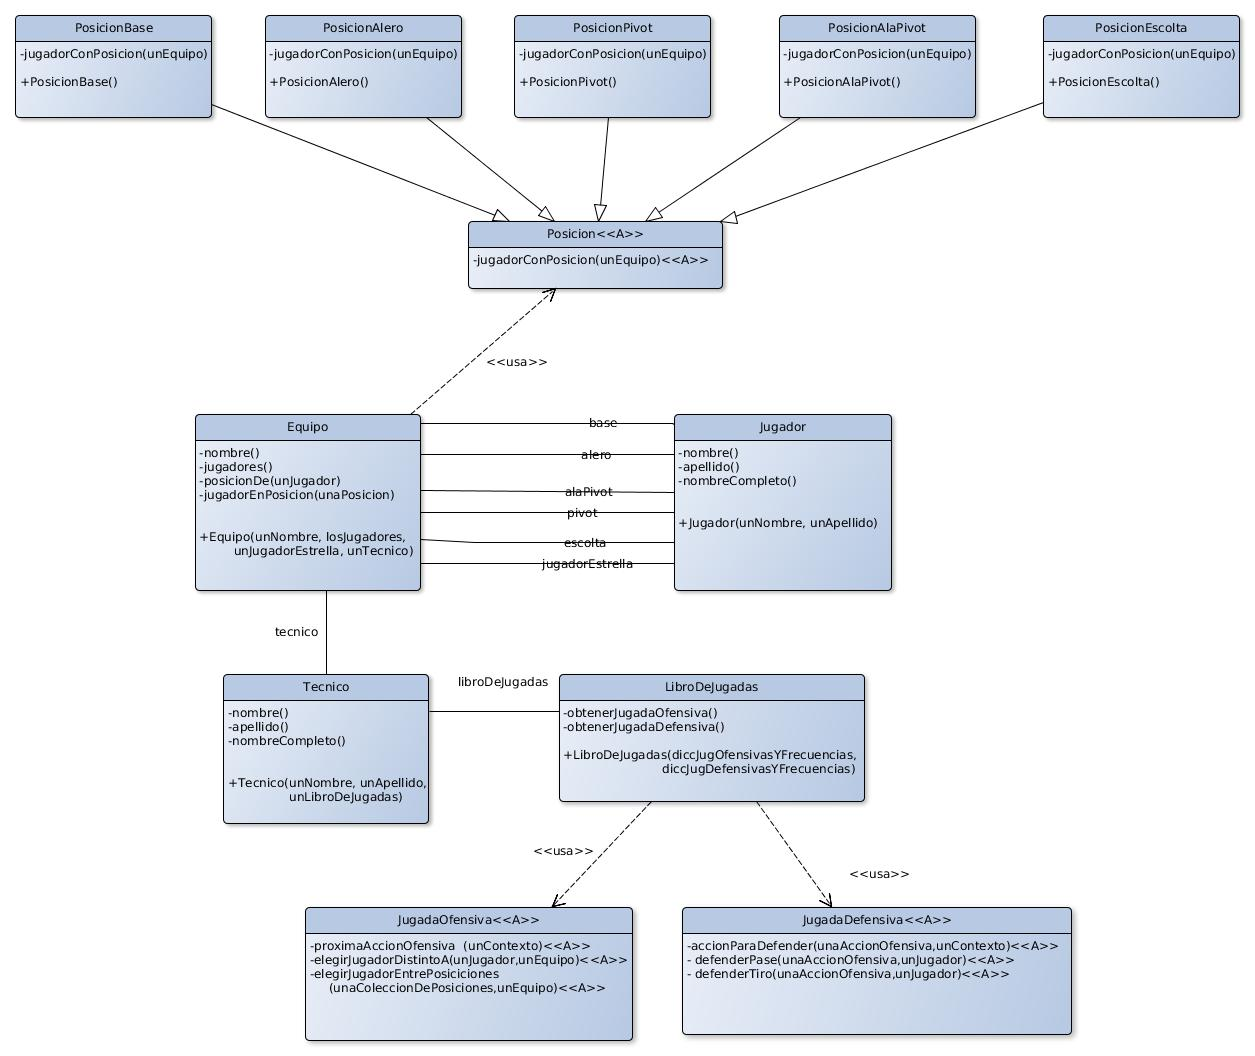
\includegraphics[scale=0.30]{diseno/equipo.jpg} 
\end{center}

A continuación veremos como se integran el tecnico con su libro de jugadas para elegir una jugada (en este caso, una ofensiva) con la simulación. Notese que, dado que las jugadas se eligen en base a la frecuencia de las mismas, se necesito de un generador de numeros aleatorios para simular el comportamiento de aleatoriedad en la eleccion de las mismas.
\begin{center}
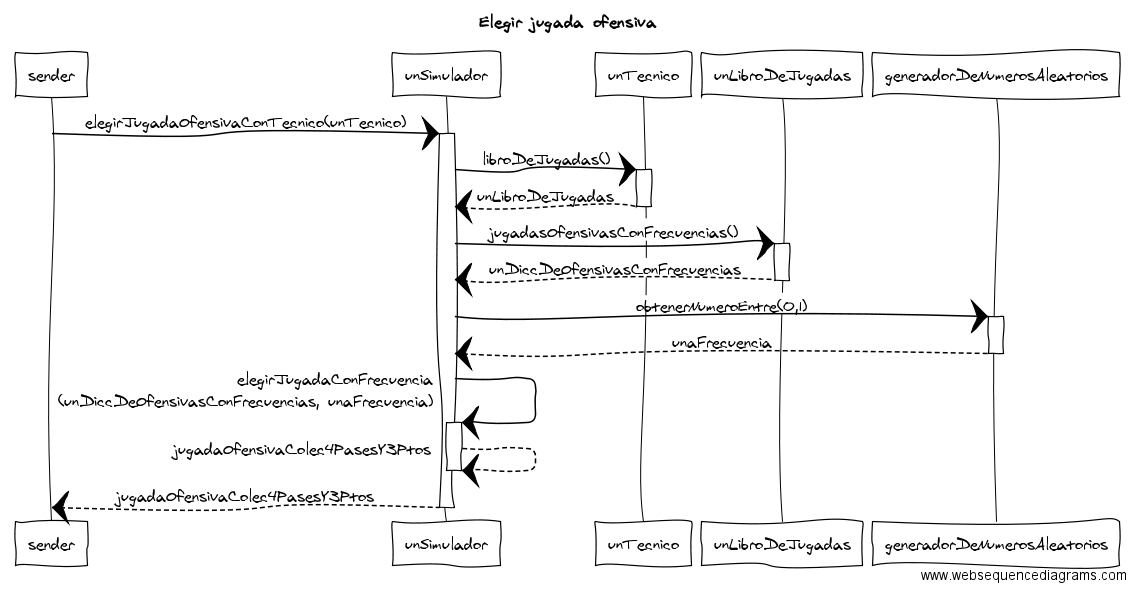
\includegraphics[scale=0.30]{diseno/Elegir_jugada_ofensiva.png} 
\end{center}

\subsection{Gestor de Equipos}
El gesto de equipos es aquel encargado de dar de alta y realizar cada una de las validaciones necesarias para confirmar la creacion de un equipo. Es por eso que se necesita de un gestor de Cap y una entidad que represente una lista de cada uno de los posibles jugadores. Esta elección nos permite disminuir la cohesión del modelo, permitiendo asi que futuras validaciones o modificaciones a las ya existentes, se agreguen de forma simple y sin agregar complejidad.
\begin{center}
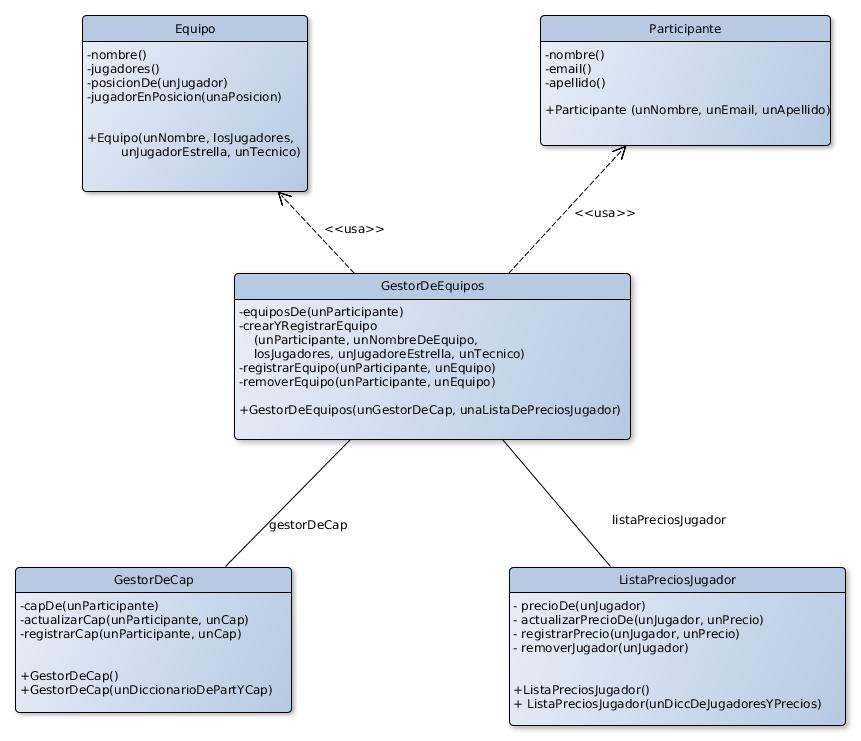
\includegraphics[scale=0.4]{diseno/gestorDeEquipos.jpg}
\end{center}

\subsection{Registro de estadisticas}
Por ultimo, decidimos contar con una entidad encargada de llevar un registro de las estadisticas de cada uno de los jugadores porque no tenia sentido que un jugador sepa responder sus estadisticas. Esto nos permitia modelar la realidad de forma mas fehaciente, dejando abierta la posibilidad de cambios en las estadisticas de forma limpia para el futuro.
\begin{center}
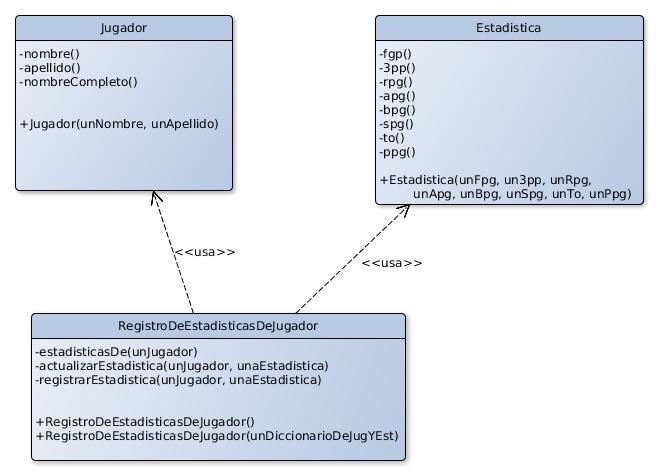
\includegraphics[scale=0.4]{diseno/registroDeEstadisticas.jpg}
\end{center}

\subsection{Partido}
Analicemos ahora el diagrama de clases de las entidades que componen un partido podemos ver, en un planteo un poco mas general, como se realiza tambien el loggeo de las distintas acciones que realizan los jugadores y como se integra la entidad resultado para poder dar cuenta de como finalizan las distintas acciones que mencionamos en secciones anteriores. Todo el loggeo de las distintas acciones se realiza mediante una clase abstracta que permite que, en un futuro en lugar de imprimir la salida por consola como sucede actualmente, la forma de logear los resultados pueda ser alterada con un minimo impacto en el resto del sistema, disminuyendo la complejidad.
\begin{center}
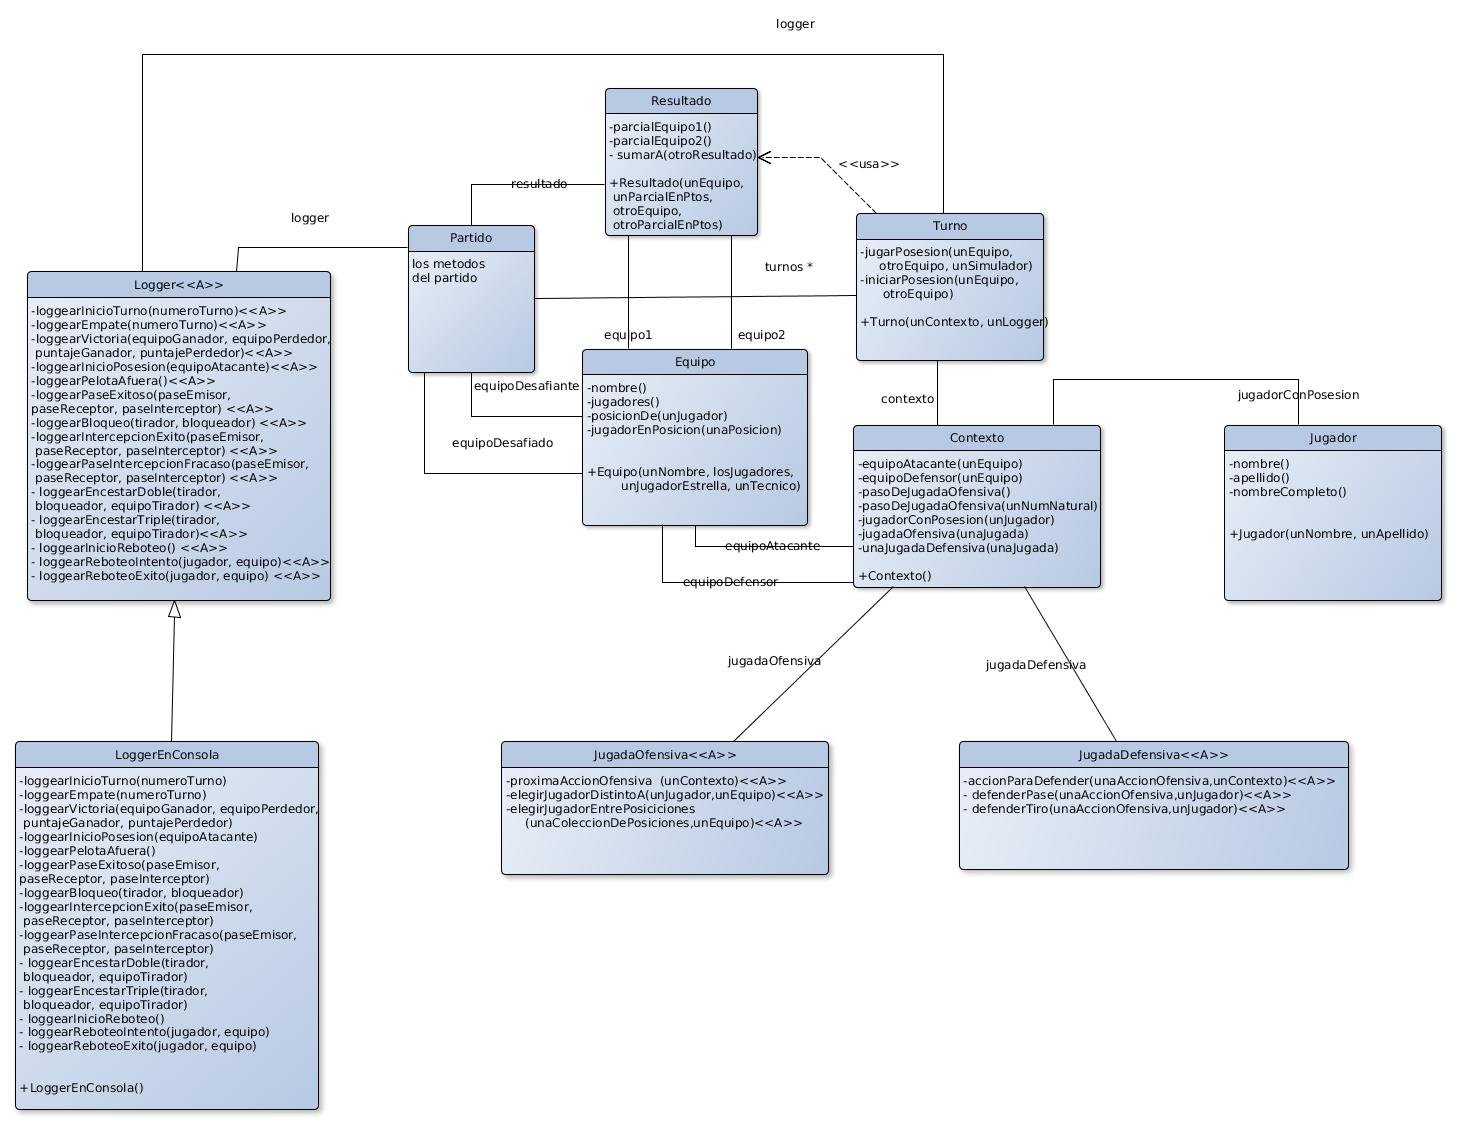
\includegraphics[scale=0.4, angle=90]{diseno/partido.jpg}
\end{center}

